\documentclass{article}
% The papersize is set to 300bp x 300bp, which will
% make the MediaBox equal [0 0 300 300].
\usepackage[papersize=300bp,margin=0pt,noheadfoot]{geometry}
\usepackage{tikz}
\pagestyle{empty}
% No compression; PDF version still might be 1.5.
\pdfcompresslevel=0
\pdfobjcompresslevel=0
\setlength{\parindent}{0pt}
\begin{document}
\pdfpageattr{%
% Enable or disable each of the following lines.
/CropBox [30 30 190 200]
/BleedBox [5 45 170 210]
/TrimBox [70 20 220 180]
/ArtBox [60 10 140 220]
}
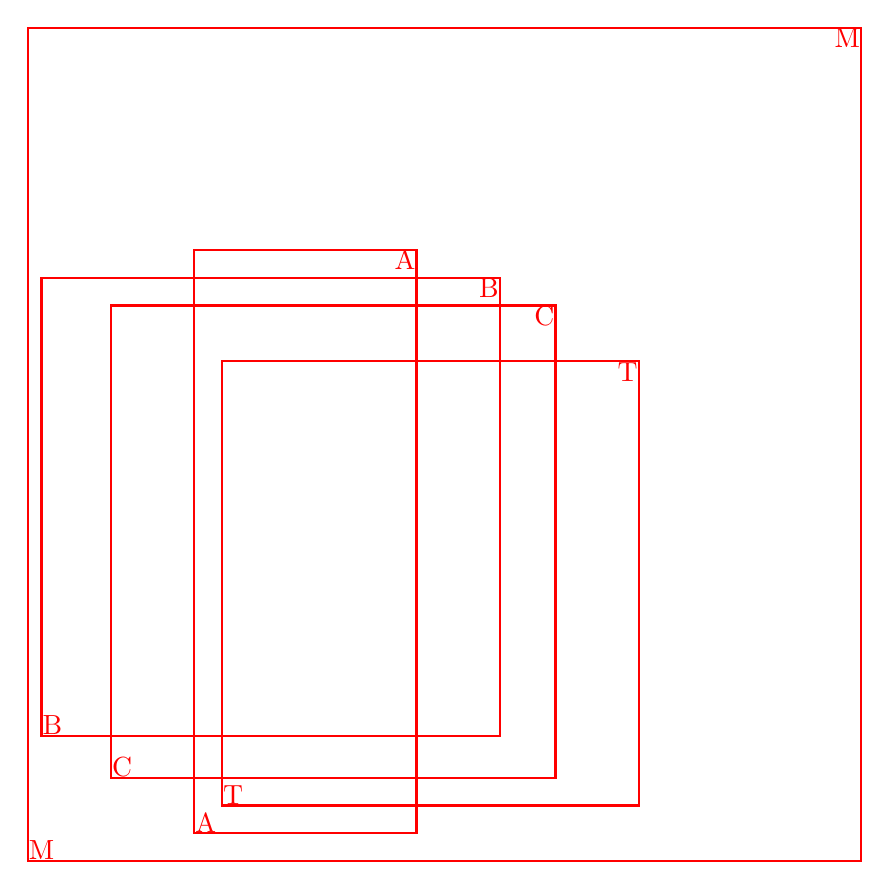
\begin{tikzpicture}[x=1bp,y=1bp,inner sep=0pt,color=red,thick]
\useasboundingbox(0,0) rectangle (300,300);
\draw (0,0) node[anchor=south west] {M} rectangle (300,300) node[anchor=north east] {M};
% Enable or disable each of the following lines.
\draw (30,30) node[anchor=south west] {C} rectangle (190,200) node[anchor=north east] {C};
\draw ( 5,45) node[anchor=south west] {B} rectangle (170,210) node[anchor=north east] {B};
\draw (70,20) node[anchor=south west] {T} rectangle (220,180) node[anchor=north east] {T};
\draw (60,10) node[anchor=south west] {A} rectangle (140,220) node[anchor=north east] {A};
\end{tikzpicture}
\end{document}
